\newpage

\section{Detekcja znaczników twarzy} \label{section:landmarks}

\textit{Facemarks} (lub \textit{Face landmarks}) to punkty nakładane na twarz wokół interesujących obszarów - takich jak oczy, nos czy usta. Pozwalają określić położenie, rozmiar czy kształt tych obiektów. Mogą być również użyte do predykcji czy mamy zamknięte/otwarte oczy (rozdz.~\hyperref[section:EARsection]{\ref{section:EARsection}}) lub czy się uśmiechamy. 

\begin{figure}[!h]
    \begin{center}
        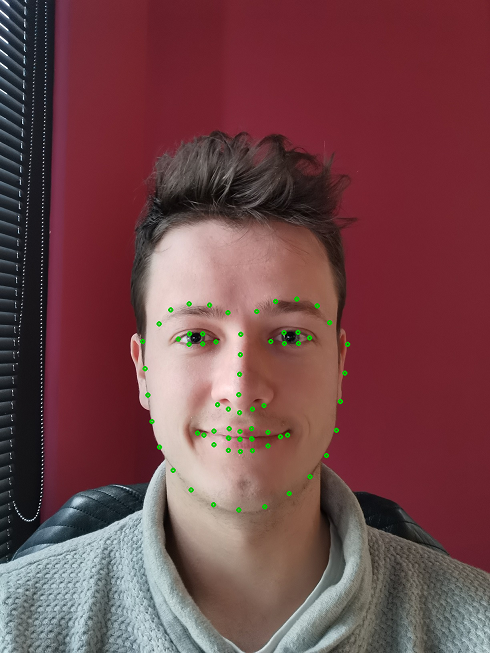
\includegraphics[scale=0.6]{img/landmark_section/landmarks_1.png}
        \caption{Przykład zdjęcia z naniesionymi punktami charakterystycznymi twarzy.}
        \label{fig:landmarks_1}
    \end{center}
\end{figure}



\subsection{Algorytmy detekcji znaczników twarzy}

Dla celów badawczych i porównania zaimplementowano dwa algorytmy, które służą do detekcji punktów charakterystycznych twarzy.


\subsubsection{Local binary features}

Metoda oparta o~\textit{histogram LBF} \cite{lbpFacemark}. W~projekcie została użyta implementacja tego algorytmu z~modułu \textit{face} \cite{opencvcontribface} zawartego w~dodatkach do biblioteki OpenCV (rozdz.~\ref{section:opencv_contrib}). Do jej działania wykorzystywany jest gotowy model \cite{lbpfacemarkmodel}, który był trenowany na datasecie \textit{HELEN} \cite{helen_dataset}.


\subsubsection{Kazemi}

Kolejnym algorytmem służącym do estymacji znaczników jest \textit{Kazemi} \cite{kazemi}, który wykorzystuje drzewa regresyjne. Jest on zaimplementowany w bibliotece dlib. Gotowy model był trenowany na podstawie zbioru danych \textit{iBUG 300-W face landmark} \cite{300Ibugdataset}.


